\subsection{Closed Loop}
\label{sec:closed_loop}
\begin{figure*}
\centering
%\vspace*{-0.3cm}  
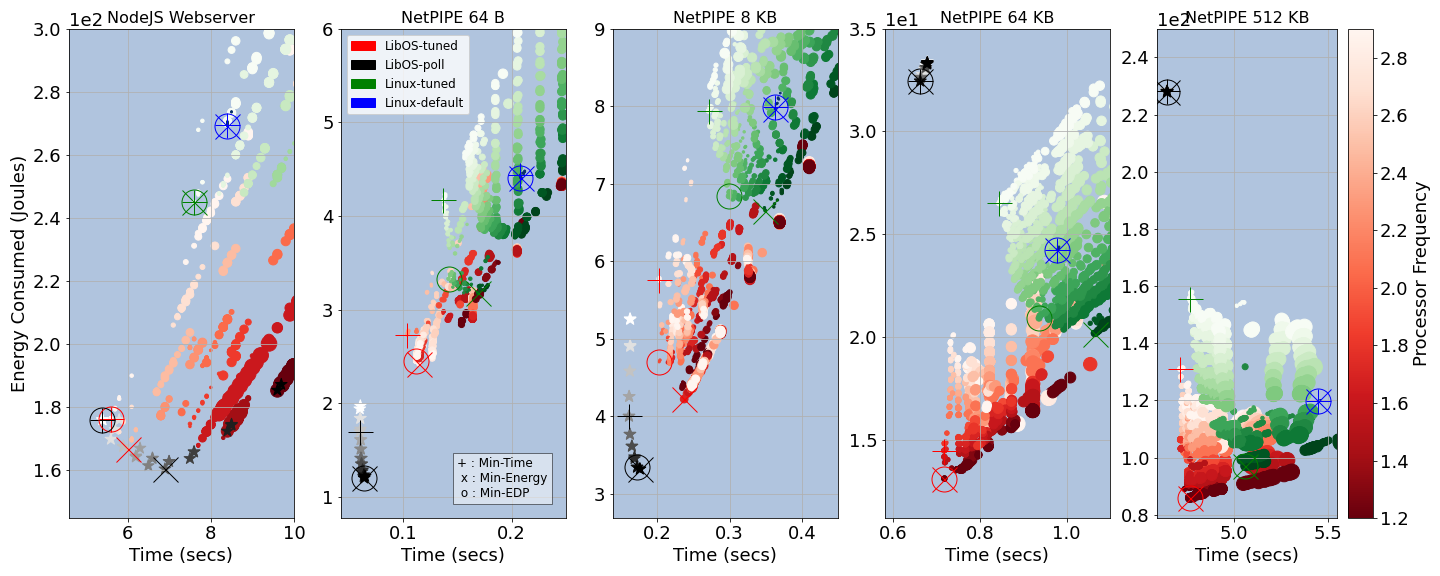
\includegraphics[width=1\textwidth]{figures/closed_loop_overview.png}
\caption[]
%{\small 
{Closed loops.}
\label{fig:closed_loop_overview}
\end{figure*}
\begin{figure*}
\centering
%\vspace*{-0.3cm}  
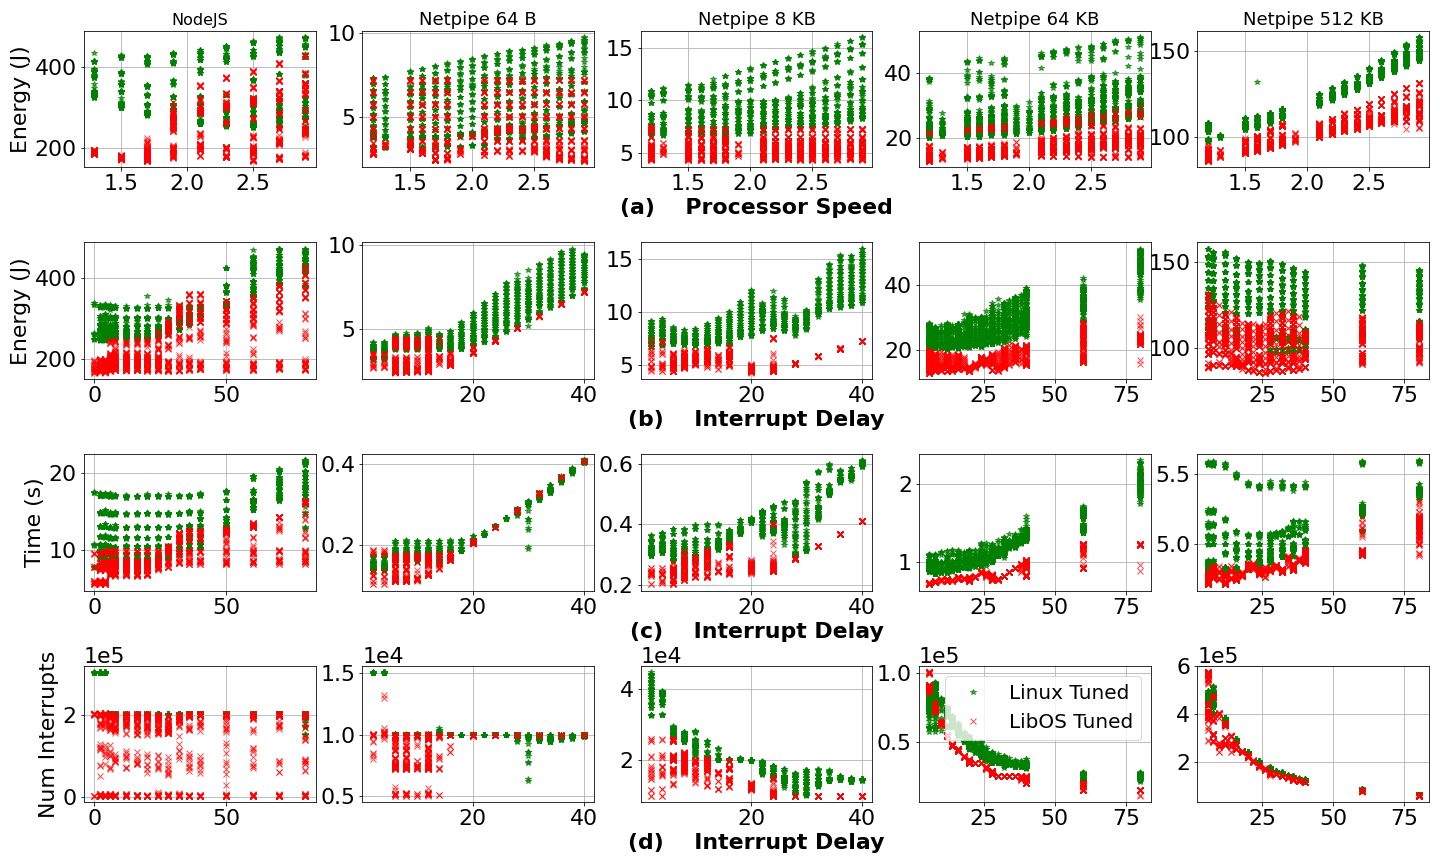
\includegraphics[width=1\textwidth]{figures/closed_detail_1.png}
\caption[]
%{\small 
{Closed loops.}
\label{fig:closed_loop_detail_1}
\end{figure*}
%This approach makes the workloads more predictable and can help smooth out diurnal variations as well~\cite{10.1145/2168836.2168842, 10.1145/2000064.2019527, oldi-study}.
% As pointed out in previous studies of energy proportionality in datacenters, the nature of web-centric applications causes diurnal troughs~\cite{Barroso:2009:DCI:1643608, oldi-study, oldi-pegasus, warehouse-power, energyproportion, WebSearch} and one method with which to increase energy efficiency during these troughs is to maximize the amount of work done, typically under a given energy budget. Figure~\ref{fig:closed_loop_overview} illustrates the set of closed-loop workloads studied in our work, all of the workloads are run in a single core with a single connection, further, they enable us to explore these simple closed-loop examples in detail in settings of computationally intensive (nodejs) and across varying network bandwidth requirements (netpipe). 

Figure~\ref{fig:closed_loop_overview} illustrates the set of closed-loop workloads studied in our work, all of the workloads are run in a single core with a single connection. Netpipe~\cite{snell1996netpipe} involves sending messages of identical size between two systems for a fixed number of iterations. We fix the iteration count at 5000 and show results for a range of message sizes. As message size increases, the workload becomes more network bound; further, linux suffers an additional memory copy from kernel to userspace compared to the libOS. Linux runs NetPIPE-3.7.1 while the libOS uses a custom version ported to its interfaces. \footnote{We found that the 10 GB link is close to saturation when a message of size greater 700 KB is exchanged.}. NodeJS~\cite{nodejs} consists a JavaScript HTTP Webserver running in side a nodejs runtime. A single client running the \textit{wrk-4.0.2}~\cite{wrk} benchmark\footnote{We modified \textit{wrk} to place a fixed request load of 100K.} sends web requests to the nodejs server for a fixed period of time. The server responds to each request with a small static payload of size 148 bytes. Linux runs nodejs-0.10.46 and library OS ported the same version to support bare-metal nodejs by providing OS interfaces that link with the V8~\cite{v8} JavaScript engine and libuv~\cite{libuv}. 

As datacenter energy use continue to rise~\cite{gupta2020chasing, NLP-energy,warehouse-power}, we believe traditional metrics such as energy-delay-product (EDP), coined from architecture community~\cite{573184,10.1109/40.888701}, should be elevated when studying efficiency of web-centric applications and systems. Therefore, we believe it is an apt metric to use when understanding these trade-offs between the various system types in a closed loop setting. We use the {\larger[4]\textbf{o}} graphical indicator in the figures below to represent the setting with best (lowest) EDP.

%We believe these set of workloads will help to simplify the complexity which to compare and contrast the effects of slowing down in the four types of systems listed above.

%\subsubsection{Observation-1: Computationally heavy applications exhibits more performance-energy trade-offs}
%Comparing the nodejs and netpipe workloads in figure~\ref{fig:closed_loop_overview}, one can see the differences in trade-offs as processor is slowed. In netpipe, the \textit{vertical-ness} as the datapoints get darker shows that slowing down the processor does not cause an increase in time, whereas the opposite is shown in the nodejs data.

% MIN-TIME linux_default   1 3.0 8.396 269.4
% MIN-TIME linux_tuned     2 2.9 7.599 244.93

% MIN-TIME linux_default 64 1 3.0 0.21 4.44
% MIN-TIME linux_tuned   64 2 2.9 0.14 4.17

% MIN-TIME linux_default 8192 1 3.0 0.36 7.99
% MIN-TIME linux_tuned   8192 8 2.8 0.27 7.94

% MIN-TIME linux_default 65536 1 3.0 0.98 24.25
% MIN-TIME linux_tuned   65536 8 2.9 0.84 26.5

% MIN-TIME linux_default 524288 1 3.0 5.45 119.77
% MIN-TIME linux_tuned   524288 8 2.9 4.77 155.56

% MIN-TIME ebbrt_tuned   4 2.9 5.6 176.11 986.11
% MIN-TIME ebbrt_poll    0 2.9 5.4 176.01 950.1

% MIN-TIME ebbrt_tuned 64 2 2.3 0.1 2.73 0.28
% MIN-TIME ebbrt_poll  64 0 2.5 0.06 1.7 0.1

% MIN-TIME ebbrt_tuned 8192 6 2.9 0.2 5.76 1.16
% MIN-TIME ebbrt_poll  8192 0 2.1 0.16 4.0 0.64

% MIN-TIME ebbrt_tuned 65536 6 1.7 0.72 14.46 10.35
% MIN-TIME ebbrt_poll  65536 6 1.3 0.66 32.45 21.48

% MIN-TIME ebbrt_tuned 524288 6 2.9 4.72 130.94 617.38
% MIN-TIME ebbrt_poll  524288 6 2.7 4.64 228.13 1059.59



% MIN-EDP linux_default 1 3.0 8.4 269.27 2261.6
% MIN-EDP linux_tuned   2 2.9 7.6 244.93 1861.22

% MIN-EDP linux_default 64 1 3.0 0.21 4.41 0.92
% MIN-EDP linux_tuned   64 2 2.1 0.14 3.33 0.47

% MIN-EDP linux_default 8192 1 3.0 0.36 7.99 2.89
% MIN-EDP linux_tuned   8192 10 2.0 0.3 6.84 2.05

% MIN-EDP linux_default 65536 1 3.0 0.98 24.25 23.72
% MIN-EDP linux_tuned   65536 12 1.8 0.94 20.91 19.57

% MIN-EDP linux_default 524288 1 3.0 5.45 119.77 652.63
% MIN-EDP linux_tuned   524288 28 1.2 5.06 97.04 491.22


% MIN-EDP ebbrt_tuned   4 2.9 5.6 176.11 986.11
% MIN-EDP ebbrt_poll    0 2.9 5.4 175.93 949.67

% MIN-EDP ebbrt_tuned   64 6 2.9 0.11 2.45 0.27
% MIN-EDP ebbrt_poll    64 0 1.2 0.06 1.2 0.08

% MIN-EDP ebbrt_tuned 8192 2 1.9 0.2 4.7 0.95
% MIN-EDP ebbrt_poll  8192 0 1.3 0.17 3.34 0.57

% MIN-EDP ebbrt_tuned 65536 6 1.2 0.72 13.07 9.37
% MIN-EDP ebbrt_poll  65536 6 1.3 0.66 32.45 21.48

% MIN-EDP ebbrt_tuned 524288 26 1.2 4.77 85.94 409.68
% MIN-EDP ebbrt_poll  524288 6 1.5 4.65 227.86 1058.57

% find configurations in which the OS interacts with slowing down to improve both time and energy. 
\subsubsection{Speeding up to save energy}
\label{sec:closed_loop:speedup}
%% relation between quiescent and time to do work
As discussed in section~\ref{sec:workflow:closed_loop}, figures~\ref{fig:closed_loop_overview} demonstrates the correlation that minimizing the time to finish the work and also results in most energy savings. One mechanism to reduce time across all the closed loop workloads and system types is to speed up interrupt delays (set a low interrupt delay value) as shown in figure~\ref{fig:closed_loop_detail_1}(c); while slow down processor does cause fluctuations in time for each interrupt delay value, the overall trend is low interrupt delay results in lowest time. By reducing time, one also minimizes energy as shown in figure~\ref{fig:closed_loop_detail_1}(b). For nodejs and netpipe 64B, we found setting a low interrupt delay (2$\mu$s)also results in the lowest EDP, this due to the lightweight nature of the payloads themselves (under a single MTU). However, as the payload sizes increase (to 8KB, 64KB, and 512KB), we found the interrupt delay value that yields best EDP also become larger, up to 28$\mu$s. A 10 GbE NIC, assuming no network jitter and switching cost, can transmit at an optimal rate of 1250 bytes/$\mu$s. Setting a static interrupt delay value is effectively determining how much payload the software should process in some fixed quantum. With larger message sizes, one can imagine portions of its payload being transmitted over the wire and processed by software asynchronously. The interrupt delay value that yields best EDP is indicating an optimal configuration with which the software should pace packet processing and save energy by sleeping during the its quiescent periods. By modulating interrupt delay, Linux-tuned improves its EDP over Linux-default by 21\%-80\%. Due to the OS path length efficiency of the libOS (see figure~\ref{fig:closed_loop_detail_1}), we find the libOS always use fewer instructions, even in computationally heavy workloads such as nodejs (7.2\% less), this efficiency coupled with a custom interrupt delay enables the libOS-tuned to achieve up to 2X better EDP than Linux-tuned.

%One can also notice the wider variation in time for nodejs in figure~\ref{fig:closed_loop_detail_1}(c), this is mainly the result of greater performance-energy trade-offs that occur in a computationally bound application.

\subsubsection{Slow-to-stay-busy effect}
In the library OS, we find slowing down of the processor results in a new energy efficient state which we term \textit{slow-to-stay-busy}. In both nodejs and netpipe 64B in figure~\ref{fig:closed_loop_detail_1}(d); for various interrupt delay values, the number of interrupts can be lowered by up to 90\%. Upon closer examination, we find slowing down of the processor causes this decrease in number of interrupts. The reason for this behavior in the library OS is described briefly in section~\ref{sec:workflow:osrepproc}; the physical transmission of OS reply packets by the network driver can occur in asynchronously with the un-winding of the stack back to the nodejs application and then down (again) to the network receive function to check for new packets. The slowing down of the processor causes this un-wind path to lengthen, potentially increasing the probability that new packets have already arrived ready to be processed by the time it reaches the network receive function. Therefore, the the software is able to skip a hardware interrupt in order to effectively stay busy and process this new reply packet. This scenario only occurs in the library OS due to the run-to-completion nature of its OS structure.
%what are configurations where this doesn't occur??

% MIN-TIME linux_default 65536 1 3.0 0.98 24.25 23.72
% MIN-TIME linux_tuned 65536 8 2.9 0.84 26.5 22.37
% MIN-TIME ebbrt_tuned 65536 6 1.7 0.72 14.46 10.35
% MIN-TIME ebbrt_poll 65536 6 1.3 0.66 32.45 21.48

% MIN-TIME linux_default 524288 1 3.0 5.45 119.77 652.63
% MIN-TIME linux_tuned 524288 8 2.9 4.77 155.56 741.87
% MIN-TIME ebbrt_tuned 524288 6 2.9 4.72 130.94 617.38
% MIN-TIME ebbrt_poll 524288 6 2.7 4.64 228.13 1059.59

\subsubsection{Trade-offs in library OS polling}
We compare the energy-performance trade-offs between slowing down the processor while the library OS is in a polling loop (LibOS-poll) and slowing down both processor and interrupt delay (LibOS-tuned). For nodejs, LibOS-poll results in a better (lower) EDP than LibOS-tuned by 4\%, this is mainly due to nodejs runtime already using a application level poll to check for new packets. Interestingly, the differences in EDP for LibOS-poll is quite dramatic as message size increases for netpipe. With 64B and 8KB message sizes, polling improves EDP by 1.6X and 3.3X respectively over LibOS-tuned. We hypothesize this is due to the smaller payload sizes, therefore getting the work done the fastest still results in the lowest energy use. In some sense, this mirrors the explanation in section~\ref{sec:closed_loop:speedup} where the best EDP for smaller payload sizes uses fast interrupt delays (an interrupt-based poll behavior). At 64KB and 512 KB, the workload becomes more network bound and our results indicate polling actually results in worse EDP by up to 2X compared to LibOS-tuned. We find at these larger message sizes sizes, polling only reduced time over LibOS-tuned by around 10\%, however energy consumption by polling was over 2X worse; which is indicative that packets spent more time on the wire than the software.

%% Vertical behavior of Netpipe 64 KB and 512 KB??